\chapter{Method}
\label{chapter:method}
\thispagestyle{empty}
\section{Proposed Watermark Attacking Pipeline}
\label{sec:pipeline}
As backgrounds and methodologies relevant to the Watermark Attacking problem have been clarified, in this section we introduce our proposed pipeline designed to address this challenge. Figure \ref{figure:overall_pipeline} provides an overview of our comprehensive pipeline, encompassing the following steps
\begin{enumerate}
 \item The original image undergoes Watermark Embedding through the Watermark Embedder. The watermark information for each image is also stored for later evaluation.
 \item The watermarked image then passes through a Watermark Localization model, revealing regional information of the watermark.
 \item The watermark is then masked from the image, creating a degraded image to be inpainted.
 \item Finally, the inpainting process, specifically I$^2$SB in our case, reconstructs the image to closely resemble the original image.
\end{enumerate}
\begin{figure}[H]
 \centering
 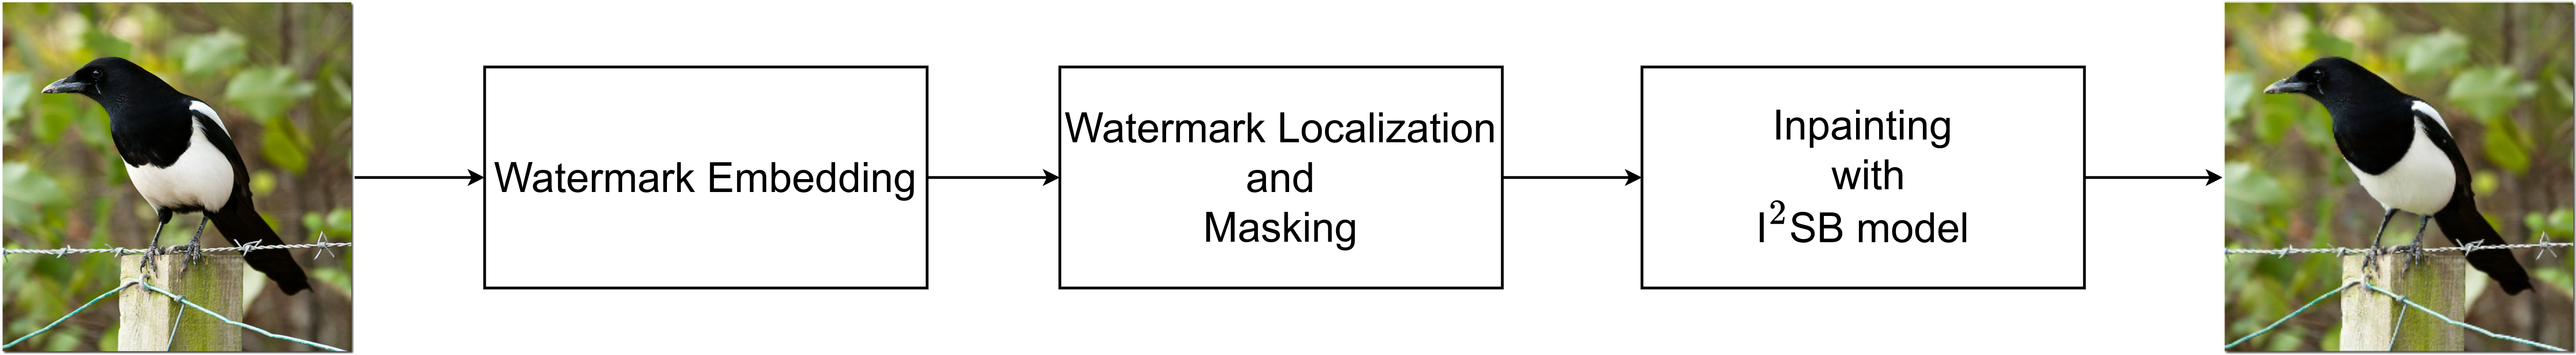
\includegraphics[width = \textwidth]{img/overall.png}
 \vspace{0.5cm}
 \caption{Overall pipeline for Watermark Attacking}
 \label{figure:overall_pipeline}
\end{figure}

% \begin{figure}[H]
%     \centering
%     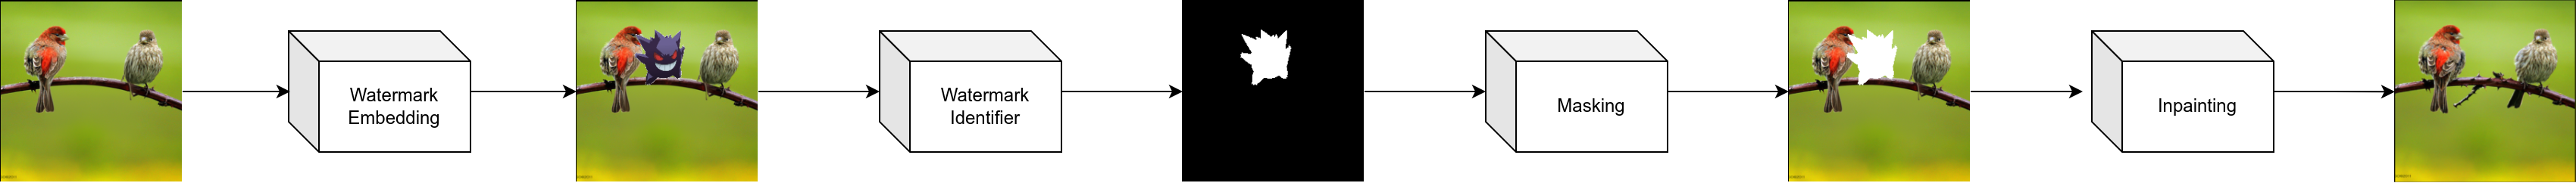
\includegraphics[width = \textwidth]{img/pipeline1.png}
%     
%     \caption{Approach 1}
%     \label{figure:appr1}
% \end{figure}

% \begin{figure}[H]
%     \centering
%     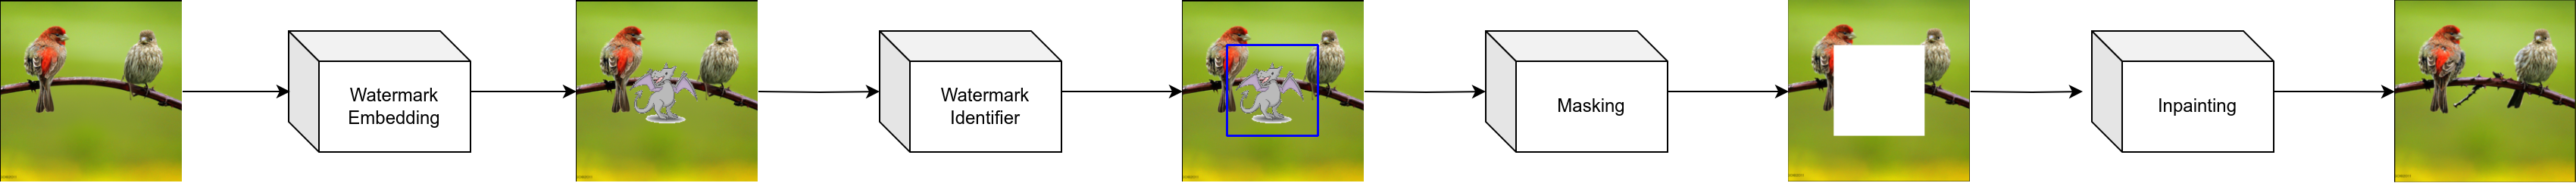
\includegraphics[width = \textwidth]{img/pipeline2.png}
%     
%     \caption{Approach 2}
%     \label{figure:appr2}
% \end{figure}
\subsection{Watermark Embedding}
\label{chapter:d:section:emb}
To begin, we will generate a watermarked dataset by embedding the watermark into the original images. Algorithm \ref{algorithm:embed} provides an overview of the watermark embedding process that we have implemented.
\begin{figure}[H]
 \centering
 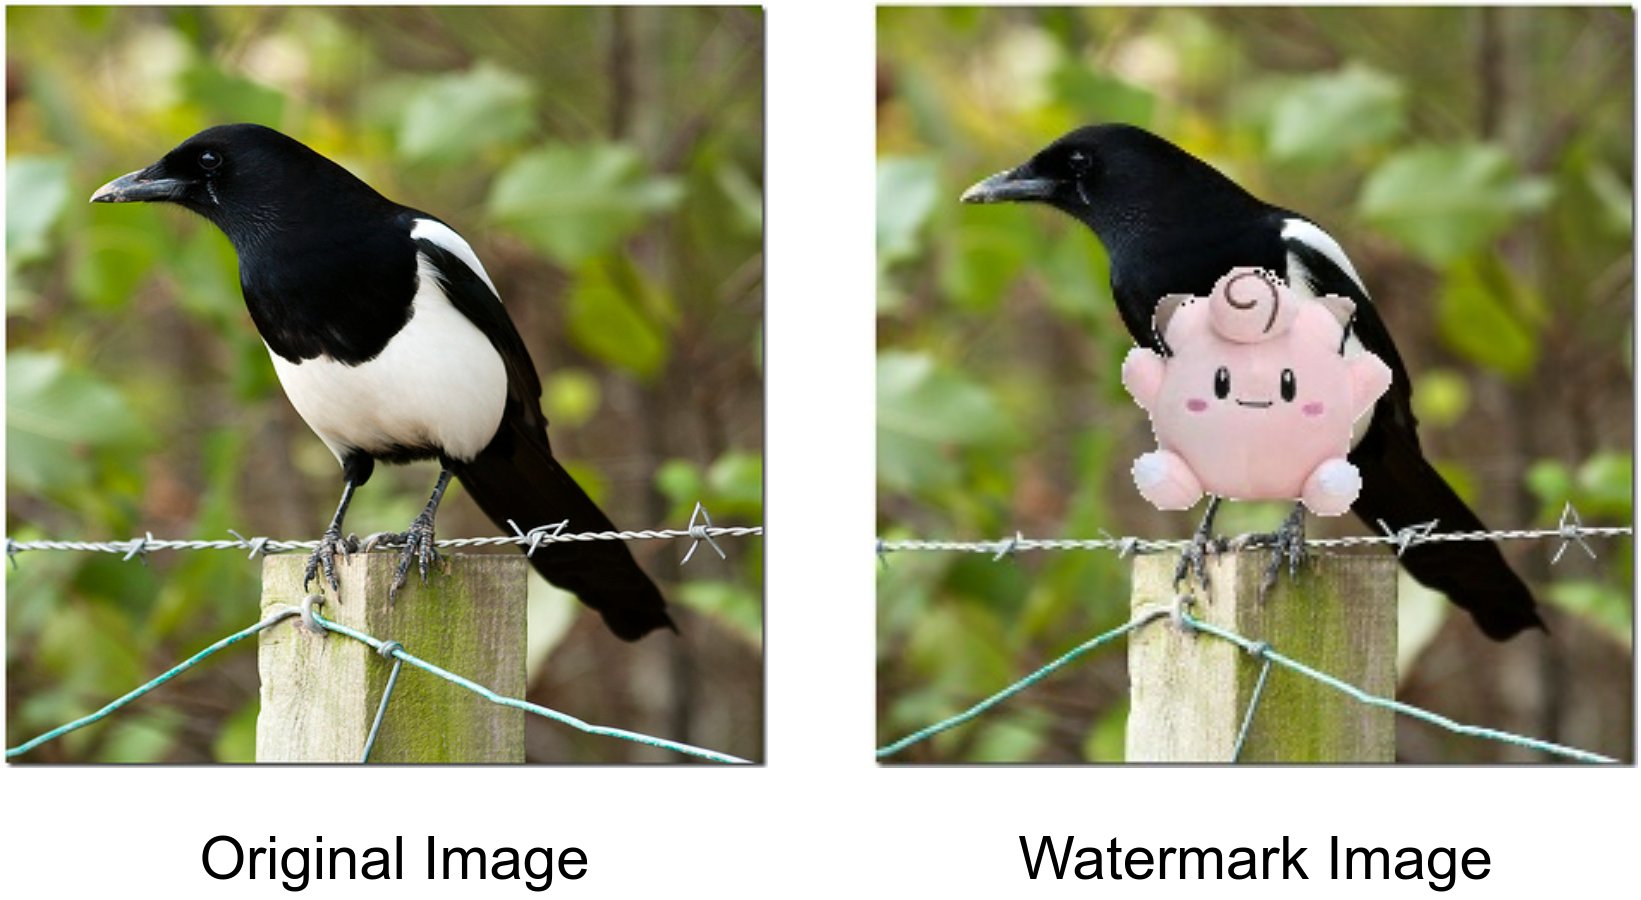
\includegraphics[width=0.75\linewidth]{img/embedded.png}

 \caption{Embed the watermark into image}
 \label{figure:embed_img}
\end{figure}
To embed the watermark, we begin with two datasets: one containing base images and the other comprising watermark images. For each image in the base dataset, we randomly select a watermark, extract its foreground using image processing, and extract the background by a specified color. For this step to be successful, it's crucial to choose a watermark dataset with minimal background detail.

The foreground of the watermark image is then placed onto the base image at a specified location, which can be either random or at the center of the image. After embedding the watermark, we save the watermarked image along with location information, such as bounding box or label map, for future reference. The resulting watermarked image is illustrated in Figure \ref{figure:embed_img}.
\begin{algorithm}[H]
 \caption{Embedding}
 \label{algorithm:embed}
 \begin{algorithmic}[1]
  \STATE {\bfseries Input:} clean dataset $A$ and watermark dataset $B$
  \FOR{$image$ {\bfseries in} $A$}
  \STATE Get random $sample$ from $B$
  \STATE Extract $foreground$ from $sample$
  \STATE Get $location$ to place watermark
  \STATE Place the $foreground$ on $location$ of $image$, save to $processed$
  \STATE Append $processed$ image to embedded dataset $C$
  \ENDFOR
  \STATE {\bfseries return} $C$
 \end{algorithmic}
\end{algorithm}
\subsection{Watermark Identifier}
After embedding and obtaining the watermarked dataset, the next step involves identifying its location information and subsequently masking it for the image inpainting task. Regarding the identifier, we plan to implement two approaches: Image Segmentation and Object Detection.
\subsubsection{Image Segmentation Approach}
In this approach, we aim to construct the watermark identifier as an object detection model. The pipeline for this approach is illustrated in Figure \ref{figure:segmentation}. There are various techniques for performing image segmentation, such as thresholding, clustering, region-based, edge-based, and graph-based methods. With the development of deep learning, many neural network architectures have been proposed for image segmentation tasks, such as U-Net, FastFCN, Gated-SCNN, and others. These architectures usually consist of an encoder and a decoder, where the encoder extracts features from the image and the decoder generates the segmentation mask. Some architectures also use additional modules or components, such as skip connections, attention mechanisms, or pyramid up-sampling, to improve the performance and accuracy of the segmentation
\begin{figure}[H]
 \centering
 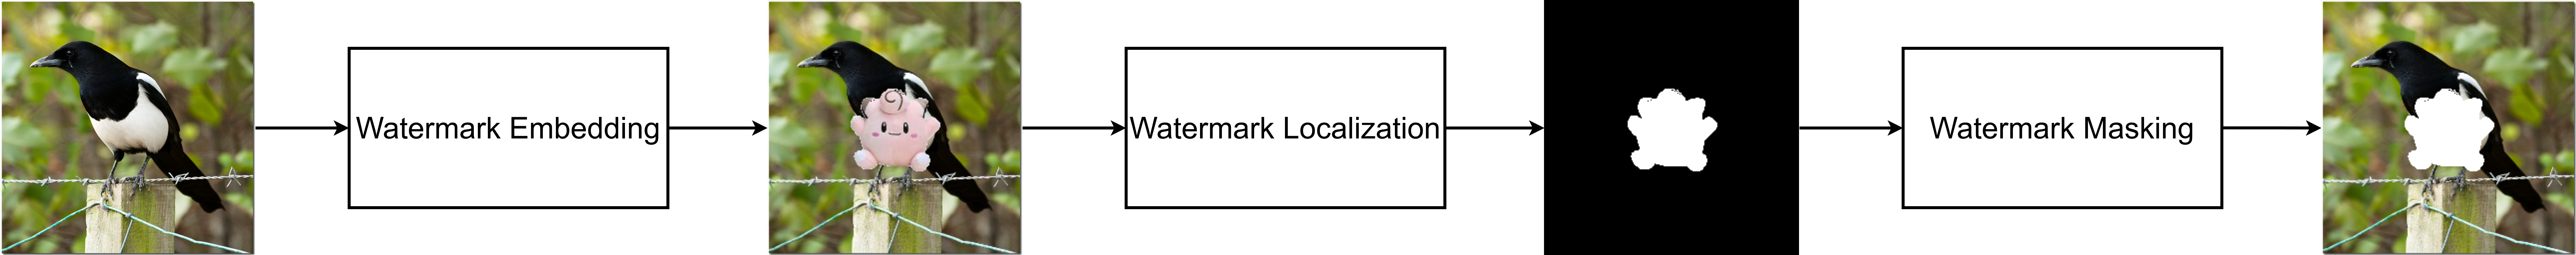
\includegraphics[width=\linewidth]{img/segmentation.png}

 \caption{Identify the watermark in image with Image Segmentation Approach}
 \label{figure:segmentation}
\end{figure}

The output of the image segmentation model is a segmentation map, with will extract the watermark out of the original image, as shown in the third image from left to right in Figure \ref{figure:segmentation}. The output from the segmentation approach provides a well-fitted segmentation for the watermark, ensuring that the mask precisely erases only the watermark during inpainting. This approach helps conserve the areas requiring inpainting, particularly those with intricate details. However, relying on segmentation introduces a strong dependency on the accuracy of the segmentation map. If the segmentation inaccurately fits the watermark, it may miss certain details, impacting the quality of the image after removing the watermark. Additionally, extending the segmentation map can be challenging, making it difficult to use the output if the watermark localization is incorrect.
\subsubsection{Object Detection Approach}
In this approach, we aim to construct the watermark identifier as an object detection model. The pipeline for this approach is illustrated in Figure \ref{figure:detection}. Object detection is a fundamental task in computer vision that aims to locate and classify objects in an image. Object detection methods can be broadly categorized into two types: two-stage detectors and one-stage detectors. Two-stage detectors first generate a set of region proposals that may contain objects, and then apply a classifier and a regressor to refine the proposals and predict the object labels and bounding boxes. One-stage detectors directly predict the object labels and bounding boxes for all the pixels or anchors in the image, without using region proposals.

Two-stage detectors are usually more accurate than one-stage detectors, but also slower and more complex. The most representative two-stage detector is the R-CNN family, which includes R-CNN, Fast R-CNN, and Faster R-CNN. R-CNN extracts features from each region proposal using a convolutional neural network (CNN), and then uses a support vector machine (SVM) and a linear regressor to classify and localize the objects. Fast R-CNN improves R-CNN by sharing the CNN features among all the region proposals, and using a softmax classifier and a bounding box regressor instead of SVM and linear regressor. Faster R-CNN further improves Fast R-CNN by replacing the selective search algorithm for generating region proposals with a region proposal network (RPN), which is a fully convolutional network that can be trained end-to-end with the detection network.

One-stage detectors are usually faster than two-stage detectors, but also less accurate and more prone to false positives. The most representative one-stage detector is the YOLO family, which now release up to YOLOv8. YOLO divides the input image into a grid of cells, and predicts the object labels and bounding boxes for each cell.

Moreover, some recent object detection methods try to bridge the gap between two-stage and one-stage detectors, by combining the advantages of both types. For example, RetinaNet  is a one-stage detector that introduces a focal loss function to address the class imbalance problem, which is the main cause of the lower accuracy of one-stage detectors. DERT  is a two-stage detector that uses a dynamic and efficient region transformer to generate adaptive region proposals, which can reduce the computation and memory cost of the detection network.
\begin{figure}[H]
 \centering
 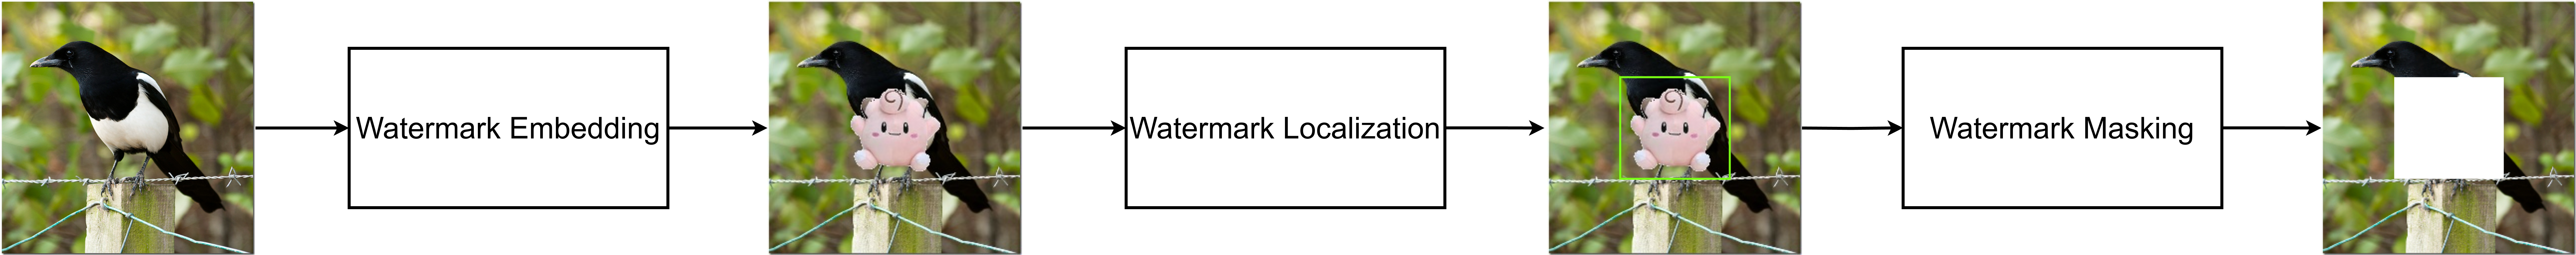
\includegraphics[width=\linewidth]{img/detection.png}

 \caption{Identify the watermark in image with Object Detection Approach}
 \label{figure:detection}
\end{figure}

The output of the object detection model is a bounding box, indicating the rectangular area where the watermark is located. Consequently, the masking area, once the box is determined, may be larger than the watermark itself. This can result in the inpainting task having to restore a larger masked area compared to the segmentation approach. However, with the location provided by the bounding box, the model's error rate may be lower than that of segmentation. This is because the segmentation approach needs to predict the exact structure of the watermark, which could be prone to missing some details.

Moreover, with the bounding box, we have the flexibility to add a padding size to the box if needed. On the contrary, extending the segmentation map can be challenging. In summary, the object detection approach makes it easier to accurately detect the location of the watermark, but the larger bounding box may pose challenges for the inpainting task.

In summary of this section, within the scope of this project, we have not yet developed a watermark identifier due to time constraints. Consequently, to execute this pipeline, we leverage the saved watermark labeling information, as discussed in Section \ref{chapter:d:section:emb}. This information is utilized for masking, enabling us to proceed directly to the image inpainting task. The development of the watermark identifier will be continued in the next phase of this project.
\subsection{Image Inpainting}
Finally, after obtaining a masked image by applying the detected watermark mask, we proceed with the inpainting task. For this task, we employ the I$^2$SB model to inpaint the masked region in the image. The process is illustrated in Figure \ref{figure:inpainting_arch}.
\begin{figure}[H]
 \centering
 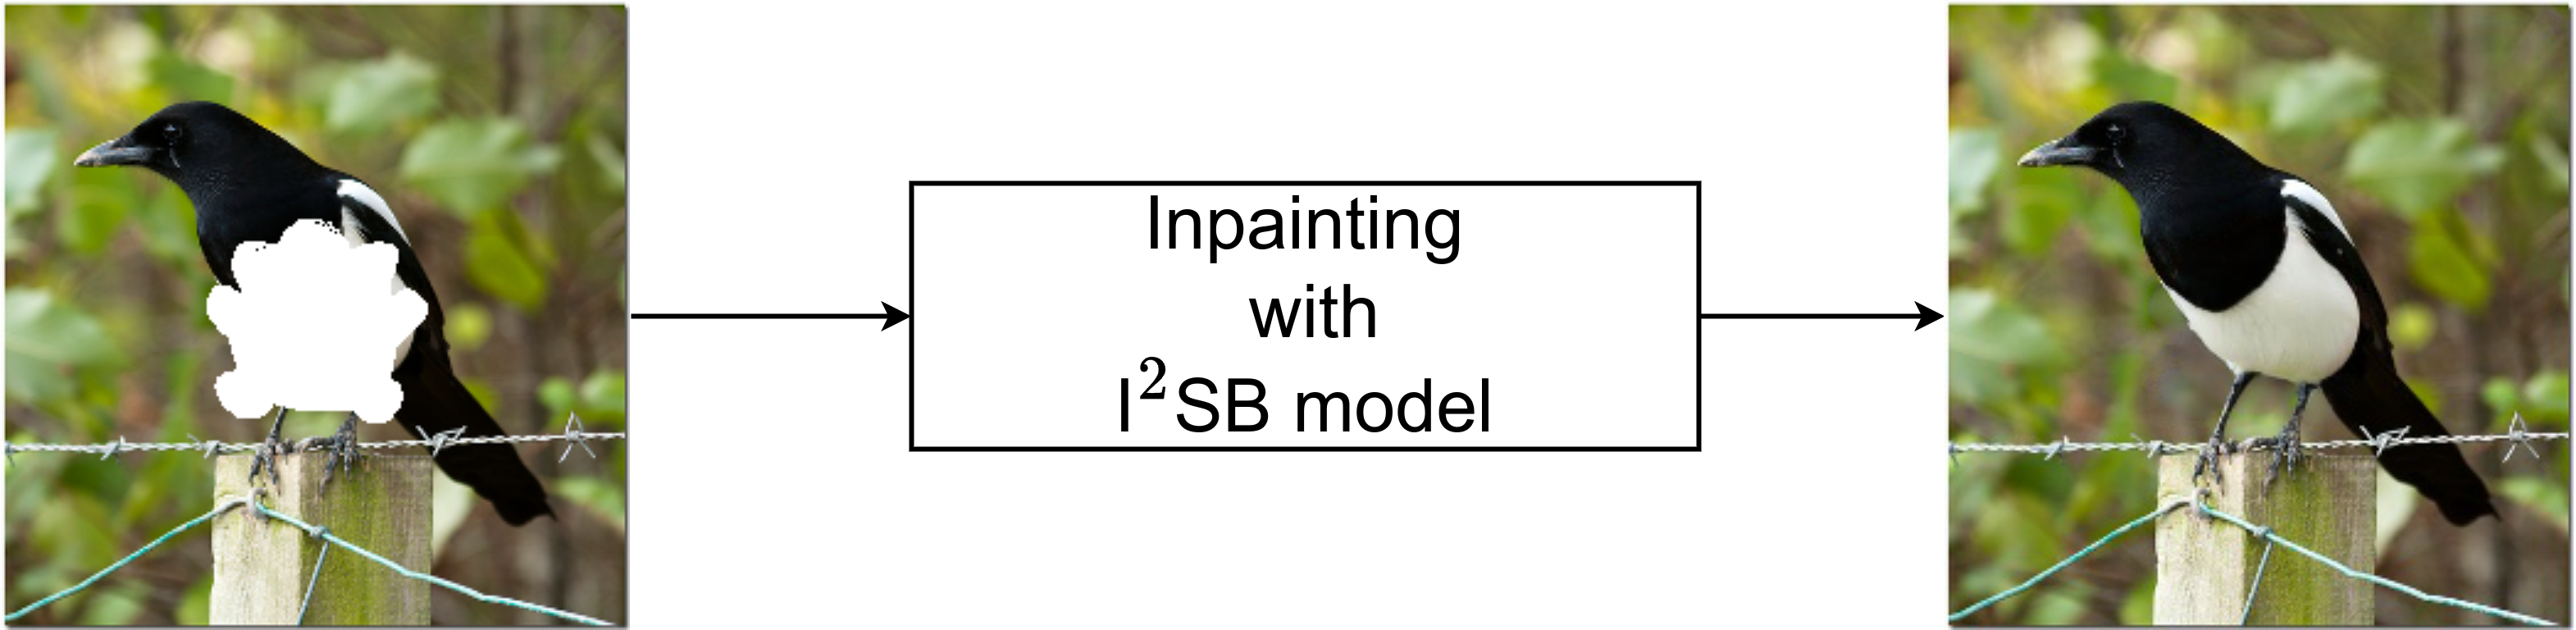
\includegraphics[width=0.75\linewidth]{img/inpainting_arch.png}

 \caption{Inpainting the mask image with I$^2$SB}
 \label{figure:inpainting_arch}
\end{figure}
The process of inpainting is explained in Figure \ref{figure:inpainting_arch}. We work with a set of details that include both the original and the covered-up image. From this information, we pick out the part of the image that's covered. The aim of this inpainting task is to bring back the covered section we've identified, hoping to recreate an image that closely resembles the original one.